
\subsection{Movimiento}
En este apartado veremos un repaso de los movimientos más básicos.


\subsubsection{MRU y MRUA}

Partiendo de la \textit{\(2^a\) Ley de Newton}, sabemos que la Fuerza es igual a la masa por su aceleración:
\[\vec{F} = m\vec{a}\]
Podemos descomponer la fuerza en sus componentes horizontales y verticales:
\[
        \vec{F_{x}}=\frac{\partial^{2}\vec{x}}{\partial{t}}m
        \to
        m\frac{\partial^2 \vec{x}}{\partial t} = 0
        \Leftrightarrow
        \frac{\partial^2{\vec{x}}}{\partial{t}} = 0
\]
\[
        \vec{F_{y}}=F_{y}\hat{\jmath}
        \to
        \vec{F_y} = m\frac{\partial\vec{v}}{\partial t}\Leftrightarrow
        \frac{\vec{F_y}}{m} = \vec{a_y}
\]
Es decir, cuando \(\vec{F_x}\) = 0N \(\to\vec{a}=0\)m/\(s^2\), por lo que la velocidad es constante, \(\vec{v}=cte\), solo si \(\vec{F_y}\neq 0\)N y \(\vec{a_y} = \vec{a} = \frac{\vec{F_y}}{m}=cte\).\par \vspace{0.5cm} Sabiendo esto y las expresiones de la aceleración y la velocidad, podemos definir las expresiones del \textbf{MRU} y \textbf{MRUA}: \par \vspace{0.5cm} \hspace{5cm}
\( \vec{a} = \frac{\partial \vec{v} }{\partial t}\) Y \( \vec{v} = \frac{\partial \vec{x} }{\partial t}\) \par \vspace{0.5cm} Obtenemos:
\[
        \int_{0}^{t}{\vec{a}\hspace{1mm}\partial{t}} = \int_{0}\partial{t}
        \to
        \boxed{\vec{v} = \vec{v_o} + \vec{a}t}
\]
\[
        \int_{0}^{t}{\vec{v}\hspace{1mm}\partial{t}} = \int_{0}{\partial{\vec{x}}}
        \to
        \boxed{\vec{x} = \vec{x_o} + \vec{v_0}t}
\]
\hspace{2.3cm} Si \( \vec{v} = \vec{v_o} + \vec{a}t\)
y
\( \vec{a} = cte \to\) \fbox{\(\vec{x} = \vec{x_o} + \vec{v_0}t + \frac{\vec{a}t^2}{2}\)}
\subsubsection{MCU y MCUA}
\begin{wrapfigure}{1}{6cm}
        \hspace{0.2cm}
        \hspace{0.5cm}
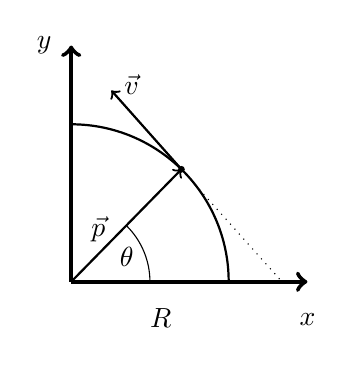
\begin{tikzpicture}[x=1cm,y=1cm]
        \draw[->,ultra thick] (0,0)--(3,0) node[above = -20]{\(x\)} node[above = -13, left = 45] {\(R\)};
        \draw[->,ultra thick] (0,0)--(0,3) node[left = 3]{\(y\)};
        \draw[thick] (2,0) arc (0:90:2);
        \draw[thin] (1,0) arc (0:45:1) node[above = -18]{\( \theta\)};
        \draw[->,thick] (1.4,1.42828) -- (0.5098765432099,2.429629629629) node[above = 2, right = 1]{\(\vec{v}\)};
        \draw[dotted] (1.4,1.42828) -- (2.676296,0);
        \draw[->,thick] (0,0) -- (1.4,1.42828) node[left = 30, above = -30]{\(\vec{p}\)};
        \filldraw[color = black] (1.4,1.42828) circle (1pt);
\end{tikzpicture}
        \par
\end{wrapfigure}
El \textbf{MCU} o Movimiento Circular Uniforme, se genera en las rotaciones de un cuerpo respecto a un punto \(p\) en un radio \(R\).
Podemos analizar la posición de un punto cualquiera, en función de las componentes horizontales y verticales:
\[
        \boxed{\vec{P}(t)=(\vec{x}(t),\vec{y}(t))=R(\cos{\theta}\vec{\imath} + \sin{\theta}\vec{\jmath})}
\]
Sabemos que el modulo de \(\vec{P}(t)\) es lo mismo que: \(\left | \vec{P} \right | = R\) y que al derivar un angulo cualquiera en función del tiempo, obtenemos la velocidad angular por unidad de tiempo: \[
        \frac{\partial \theta}{\partial t} = \frac{v}{R}t = wt\
\]
Por lo tanto, podemos concluir con lo siguiente
\[
        \vec{v} =\frac{\partial \vec{P}}{\partial t} =R \hspace{1.35mm} (w\cos{\theta}\vec{\jmath} - w\sin{\theta}\vec{\imath}\hspace{1mm})  = \boxed{Rw \hspace{1.35mm} (\cos{\theta}\vec{\jmath} - \sin{\theta}\vec{\imath}\hspace{1mm})}
\]
Y que el modulo de la velocidad es constante:
\[
        \left | \vec{v} \right | = wR = cte
\]
Evidentemente podemos calcular a partir de la velocidad, el vector aceleración:
\[
        \vec{a} =\frac{\partial \vec{v}}{\partial t} = -Rw^2 \hspace{1.35mm}(\cos{\theta}\vec{\imath} + \sin{\theta}\vec{\jmath}\hspace{1mm}) \hspace{1.35mm}= \boxed{-w^{2}\vec{P}}
\]
De esta expresón podemos deducir que \underline{el vector \(\vec{a}\) es Antiparalelo a \(\vec{P}(t)\)} y el modulo de la aceleración es \fbox{\(\left | \vec{a} \right |=\frac{v^2}{R}\)}
\subsection{Vectores}
Un vector es un elemento matemático dotado de dirección, sentido y modulo, es decir, el vector se mueve de cierta forma a un punto, de una forma concreta a una distancia.
Aquí aparecerán las operaciones y transformaciones más relevantes:


\vspace{0.5cm}
Considerando los vectores \( \vec{u},\vec{w}, \vec{u} \in \mathbb{R}^n\) tenemos:


\vspace{0.3cm}
\begin{itemize}
        \item Producto escalar: \( \vec{v}\cdot \vec{w} = \left\lvert v\right\rvert \left\lvert w\right\rvert \cos{\alpha } = \left\lvert u\right\rvert \)


        \item Producto vectorial: \(\vec{v}\times  \vec{w} = \left\lvert v\right\rvert \left\lvert w\right\rvert \sin{\alpha } = \vec{u} = \begin{vmatrix}
                      \vec{\imath} & \vec{\jmath} & \vec{k} \\
                      v_x          & v_y          & v_z     \\
                      w_x          & w_y          & w_z
              \end{vmatrix} =\) \par \hspace{1.5cm} \( = \vec{\imath}
              \begin{vmatrix}
                      v_y & v_z \\
                      w_y & w_z
              \end{vmatrix}
              -\vec{\jmath} \begin{vmatrix}
                      v_x & v_z \\
                      w_x & w_z
              \end{vmatrix}
              + \vec{k} \begin{vmatrix}
                      v_x & v_y \\
                      w_x & w_y
              \end{vmatrix}
              \) \par
              En el Tema 3, veremos algunas propiedades interesantes, sin embargo, con esto será suficiente.
        \item Vector unitario: \( \hat{u} = \frac{\vec{u}}{\left | \vec{u} \right |}\) Lo que da lugar a un vector, igual en todo sentido a \(\vec{u}\) pero de longitud 1.
\end{itemize}
%TODO COMPLETAR ESTA PARTE CUANDO SE LLEGUE AL TEMA DE CORRIENTE ALTERNA%
\subsection{Trigonometría}
%TODO INDICAR EL CALCULO DE ANGULOS, TRASLACION DE ANGULOS DE UN CUADRANTE A OTRO, PROPIEDADES DE ANGULOS AL SUMAR, RESTAR, ETC%
\subsection{Números Complejos}
%TODO EXPLICAR QUE ES UN COMPLEJO, OPERACIONES Y PROPIEDADES%
\subsubsection{Fasores}
%TODO RELACION CON LOS NUMEROS COMPLEJOS Y EL NUMERO DE EULER, CON MOBRIUS%